\documentclass[manuscript,11pt]{article}

\pagestyle{plain}                                                                            
\setlength{\textwidth}{6.5in}  
\setlength{\oddsidemargin}{0in}  
\setlength{\evensidemargin}{0in} 
\setlength{\textheight}{8.5in}      
\setlength{\topmargin}{0in}        
\setlength{\headheight}{0in}       
\setlength{\headsep}{0in}       
\setlength{\footskip}{.5in}                    

\makeatletter     
\let\@dates\relax
\makeatother

\bibliographystyle{apj}  

\newcommand{\barne}{\ensuremath{\bar{n}_e}}
\newcommand{\AU}{\ensuremath{\textrm{ AU}}}
\newcommand{\mas}{\ensuremath{\textrm{ mas}}}
\newcommand\tab[1][1cm]{\hspace*{#1}}
\usepackage{graphicx}
\graphicspath{ {images/} }
\usepackage{latexsym}
\usepackage{enumitem}
\usepackage{amssymb}
\usepackage{amsmath}
\usepackage{amsfonts}
\usepackage{float}
\usepackage{wrapfig}
\usepackage{url}
\usepackage{booktabs,caption}
\usepackage{mhchem}
\usepackage{textcomp}
\providecommand{\e}[1]{\ensuremath{\times 10^{#1}}}
%\setlength{\parindent}{0pt}
\newcommand{\forceindent}{\leavevmode{\parindent=1em\indent}}

\linespread{1}

\begin{document}

\title{\Large Project 1: Visual Question Answering}
\author{Simon Gilbert}
\maketitle 
Visual Question Answering (VQA) is a subset of machine learning in which a computer is tasked with answering questions posed by people using natural language (as opposed to coding syntax i.e.).  This is most frequently done in relation to an image an example of which is shown below in fig \ref{soccer}. A successful VQA program should be able to take in an image, a user-generated question, and be able to come up with an answer by drawing on a database of information. For example, from fig \ref{soccer}, user might ask ``how many players are there on each team?" or  ``are the players wearing shoes?" and the program has to analyze the image and provide an accurate response in a reasonable timeframe. \\

\begin{figure}[h]
\centering
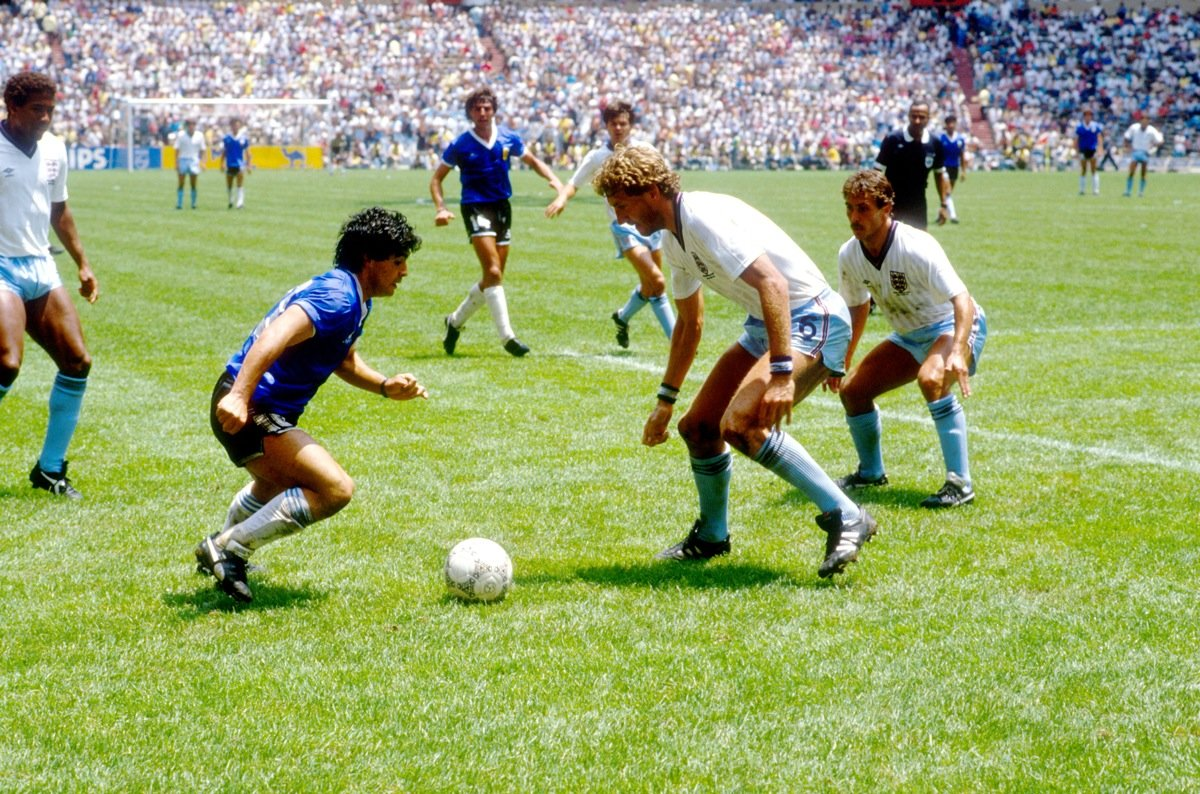
\includegraphics[scale=.8]{soccer}
\caption{A sample image on which one might want to run VQA software.}
\label{soccer}
\end{figure} 

Tasks like this are simple for humans, but creating a program capable of the same speed and accuracy as a person is a significantly more difficult undertaking. A program capable of performing such a complex task requires an ability to utilize natural language processing (NLP) to interpret the user input and provide a cogent response. It must recognize objects in images with high accuracy and also be able to efficiently search a database of information to provide an answer. Getting every step of the pipeline to work at a high level is incredibly difficult which is why VQA is at the forefront of today's most significant machine learning challenges. 
A simple approach to a VQA network architecture is shown below in figure \ref{vqaarchitecture}. First, an image is fed into a convolutional neural network (CNN) such as Resnet18 \footnote{Resnet18 would be pre-trained on an image database such as ImageNet which contains millions of images and associated descriptors.} (architecture shown in fig. \ref{resnet}), and the network outputs a feature vector which encodes the contents of the image. Next the features of the question are extracted using word2vec which captures the syntax and semantics of each word and encodes each of them in a feature vector with a specific length. Often, the embedded feature vectors for the image and question have different lengths, so a linear transformation is applied to make them the same dimension. The vectors are then point-wise multiplied and fed through a softmax layer which outputs the probability distribution over the top K answers. \\

\begin{figure}[h]
\centering
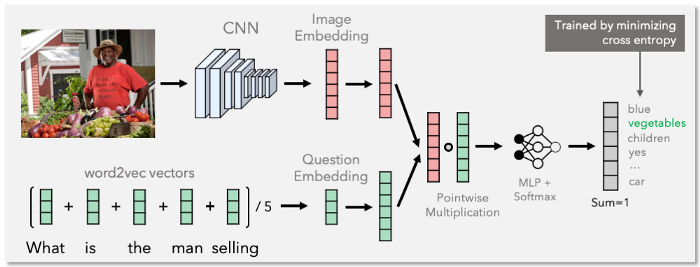
\includegraphics[scale=.5]{vqaarchitecture}
\caption{A simple VQA architecture with a convolutional neural network to process images, a module to process user input into questions, and a means for processing the two together to form an answer.}
\label{vqaarchitecture}
\end{figure} 

\begin{figure}[h]
\centering
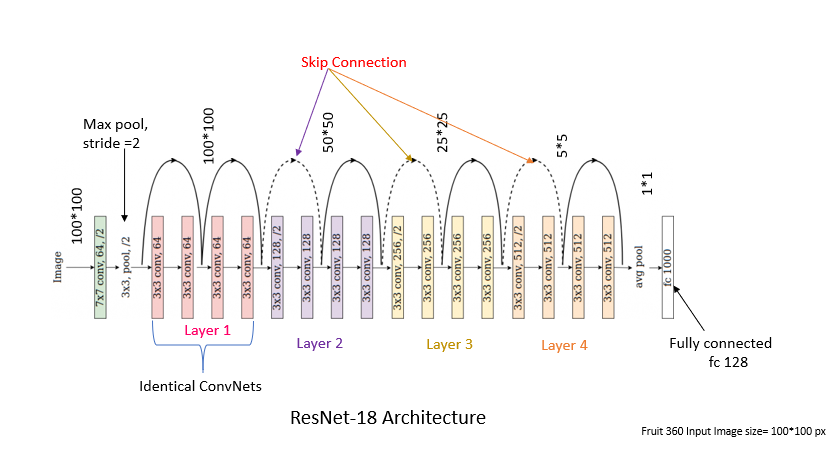
\includegraphics[scale=.5]{resnet}
\caption{The Resnet18 neural network architecture implemented in the VQA pipeline in fig 2.}
\label{resnet}
\end{figure} 

The architecture described above performs with an accuracy of 57.8\% when presented with open-ended questions on the VQA-v1 dataset\footnote{This dataset contains approximately 200,000 images and 600,000 questions with 6,000,000 ground truth answers.}. This seems impressive for such a difficult task, but we must compare this to some sort of baseline. It turns out that if you present the above architecture with just the question without the image provided, it still manages to get 50.4\% accuracy! This seems crazy, until one considers the types of questions asked of it. For example, the program might be asked ``what color is the soccer ball?". This kind of question narrows the answer-space from 1000s of potential answers down to just a few: a small range of colors. From training, the program can fairly easily learn that most soccer balls are black and white, and could therefore guess those as answers with a relatively high accuracy without ever being shown the picture in question.\\

There are several variations on the VQA architecture proposed above some of which are presented below in fig. \ref{VQAapproaches}. I am not going to go into detail about the pros and cons of each change one can make to the pipeline, but I thought it would be interesting to show here at a high level. The main idea is that most current VQA systems are broken into 3 main stages: image feature extraction, question feature extraction, and combining those features to get a result. The variations engineers can implement come at each one of these stages whether it be tweaking the convolutional neural network used for image feature extraction, using long short term memory as a different type of question encoder, or using Bayesian approaches to infer relationships between image and question features. \\

\begin{figure}[h]
\centering
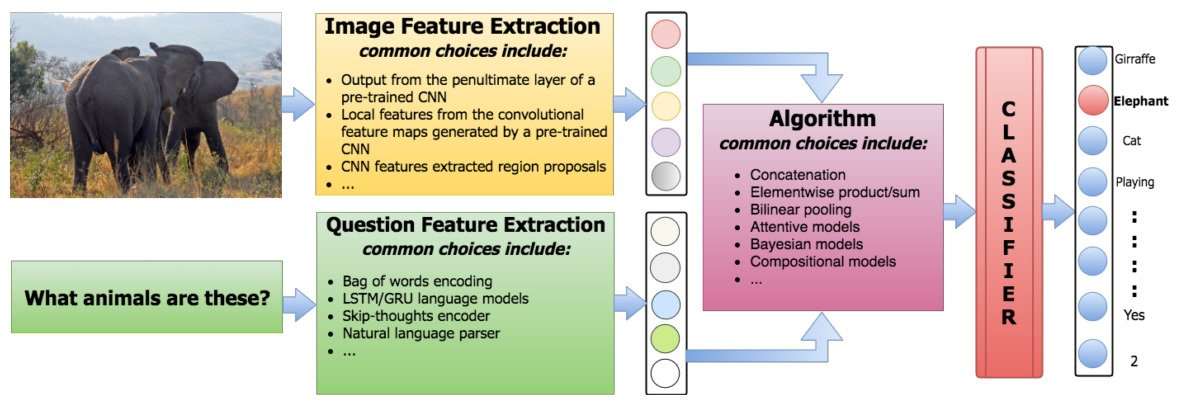
\includegraphics[scale=.3]{VQAapproaches}
\caption{Graphic showing possible modifications to the baseline VQA architecture.}
\label{VQAapproaches}
\end{figure} 

\begin{figure}
\centering
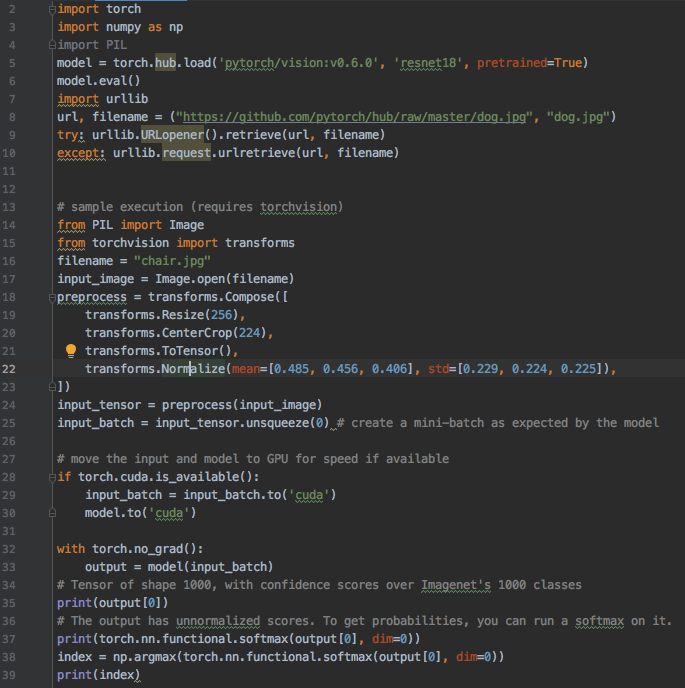
\includegraphics[scale=.35]{code}
\caption{Code for testing on a pre-trained Resnet18. Line 16 can be used to feed in an image of your choice.}
\label{code}
\end{figure} 

I tried to implement Resnet18, the neural network used in the architecture described above in fig \ref{vqaarchitecture}. I was able to download and install a pre-trained network the code for which is shown in fig \ref{code}. This code can be used to classify images into 1 of 1000 object classes, but is not able to perform question answer on that image (for that, I would need access to a GPU and a significant amount of disk space). It does, however perform very well at classifying images. For example, I fed it a picture of dog and not only was it able to identify that the image was a dog but specifically a German Sheppard! I actually thought this was super cool. I would like to eventually implement a full VQA architecture using the BU shared computing center later in the semester.

\pagebreak
\section{Bibliography}
\begin{itemize}
\item Couto, Javier. ``Introduction to Visual Question Answering: Tryolabs Blog." Introduction to Visual Question Answering | Tryolabs Blog, Tryolabs, 1 Mar. 2018, \\
tryolabs.com/blog/2018/03/01/introduction-to-visual-question-answering/. 
\item Kembhavi, A. (2019, June 13). Vanilla VQA. Retrieved September 17, 2020, from 
https://medium.com/ai2-blog/vanilla-vqa-adcaaaa94336
\item Kafle, K., \&amp; Kanan, C. (2017). Visual question answering: Datasets, algorithms, and future challenges. Computer Vision and Image Understanding, 
163, 3-20. doi:10.1016/j.cviu.2017.06.005
\item Kembhavi, A. (2020). Textbook Question Answering Challenge. Retrieved September 17, 2020, from http://vuchallenge.org/tqa.html
\item VQA. (n.d.). Retrieved September 17, 2020, from https://visualqa.org/index.html
\item Stanford University (2016). About ImageNet. Retrieved September 17, 2020, from http://www.image-net.org/about-overview
\item Pytorch Team. (n.d.). Resnet. Retrieved September 17, 2020, from \\
https://pytorch.org/hub/pytorch\_vision\_resnet/
\item Pytorch/vision. (2020, March 16). Retrieved September 17, 2020, from \\
https://github.com/pytorch/vision/blob/master/torchvision/models/resnet.py
\item Fox, E., \&amp; Guestrin, C. (n.d.). Text: Imagenet 1000 class idx to human readable labels (Fox, E., &amp; Guestrin, C. (n.d.). Coursera Machine Learning Specialization.). \\
Retrieved September 17, 2020, from https://gist.github.com/yrevar/942d3a0ac09ec9e5eb3a
\end{itemize}

\end{document}